\documentclass[a4paper, top=10mm]{article}
%for writing from the top
\usepackage{fullpage}
%for math
\usepackage{amsmath}
\usepackage{mathrsfs}
\usepackage{amsthm}
%for images
\usepackage{graphicx}
%for color
\usepackage{xcolor}
%for title
\title{\textbf{\huge{Hidden Chocolates}}}
\author{Enigma n\textsuperscript{o}3}
\date{14\textsuperscript{th} December 2023}

\newtheorem*{hint}{Hint}

\addtolength{\voffset}{-2cm}
\addtolength{\textheight}{5cm}


\begin{document}
	\maketitle
	
	Paul-Henry Cournède (PHC) and Céline Hudelot (CH) are sitting face to face.
	We tell them there are $50$ black chocolates, and $50$ white chocolates, for a total of $100$ chocolates.
	There are $50$ chocolates behind Céline, and $49$ behind Paul-Henry.
	One chocolate is hidden.
	
	The two professors can not see the chocolates behind them-self, but they can see the ones behind the other professor.
	We ask them iteratively "Do you know what is the color of the hidden chocolate?".
	
	They answer as follows:
	
	\begin{enumerate}
		\item \textbf{PHC}: "I do not know."
		\item \textbf{CH}: "I do not know."
		\item \textbf{PHC}: "I do not know."
		\item \textbf{CH}: "I do not know."
		\item \textbf{PHC}: "I do not know."
		\item \textbf{CH}: "I do not know."
		\item \textbf{PHC}: "I do not know."
		\item \textbf{CH}: "I do not know."
		\item \textbf{PHC}: "I do not know."
		\item \textbf{CH}: "I do not know."
		\item \textbf{PHC}: "I do not know."
		\item \textbf{CH}: "I do not know."
		\item \textbf{PHC}: "I do not know."
		\item \textbf{CH}: "I do not know."
		\item \textbf{PHC}: "I know! It is white!"
	\end{enumerate}
	
	\begin{center}
		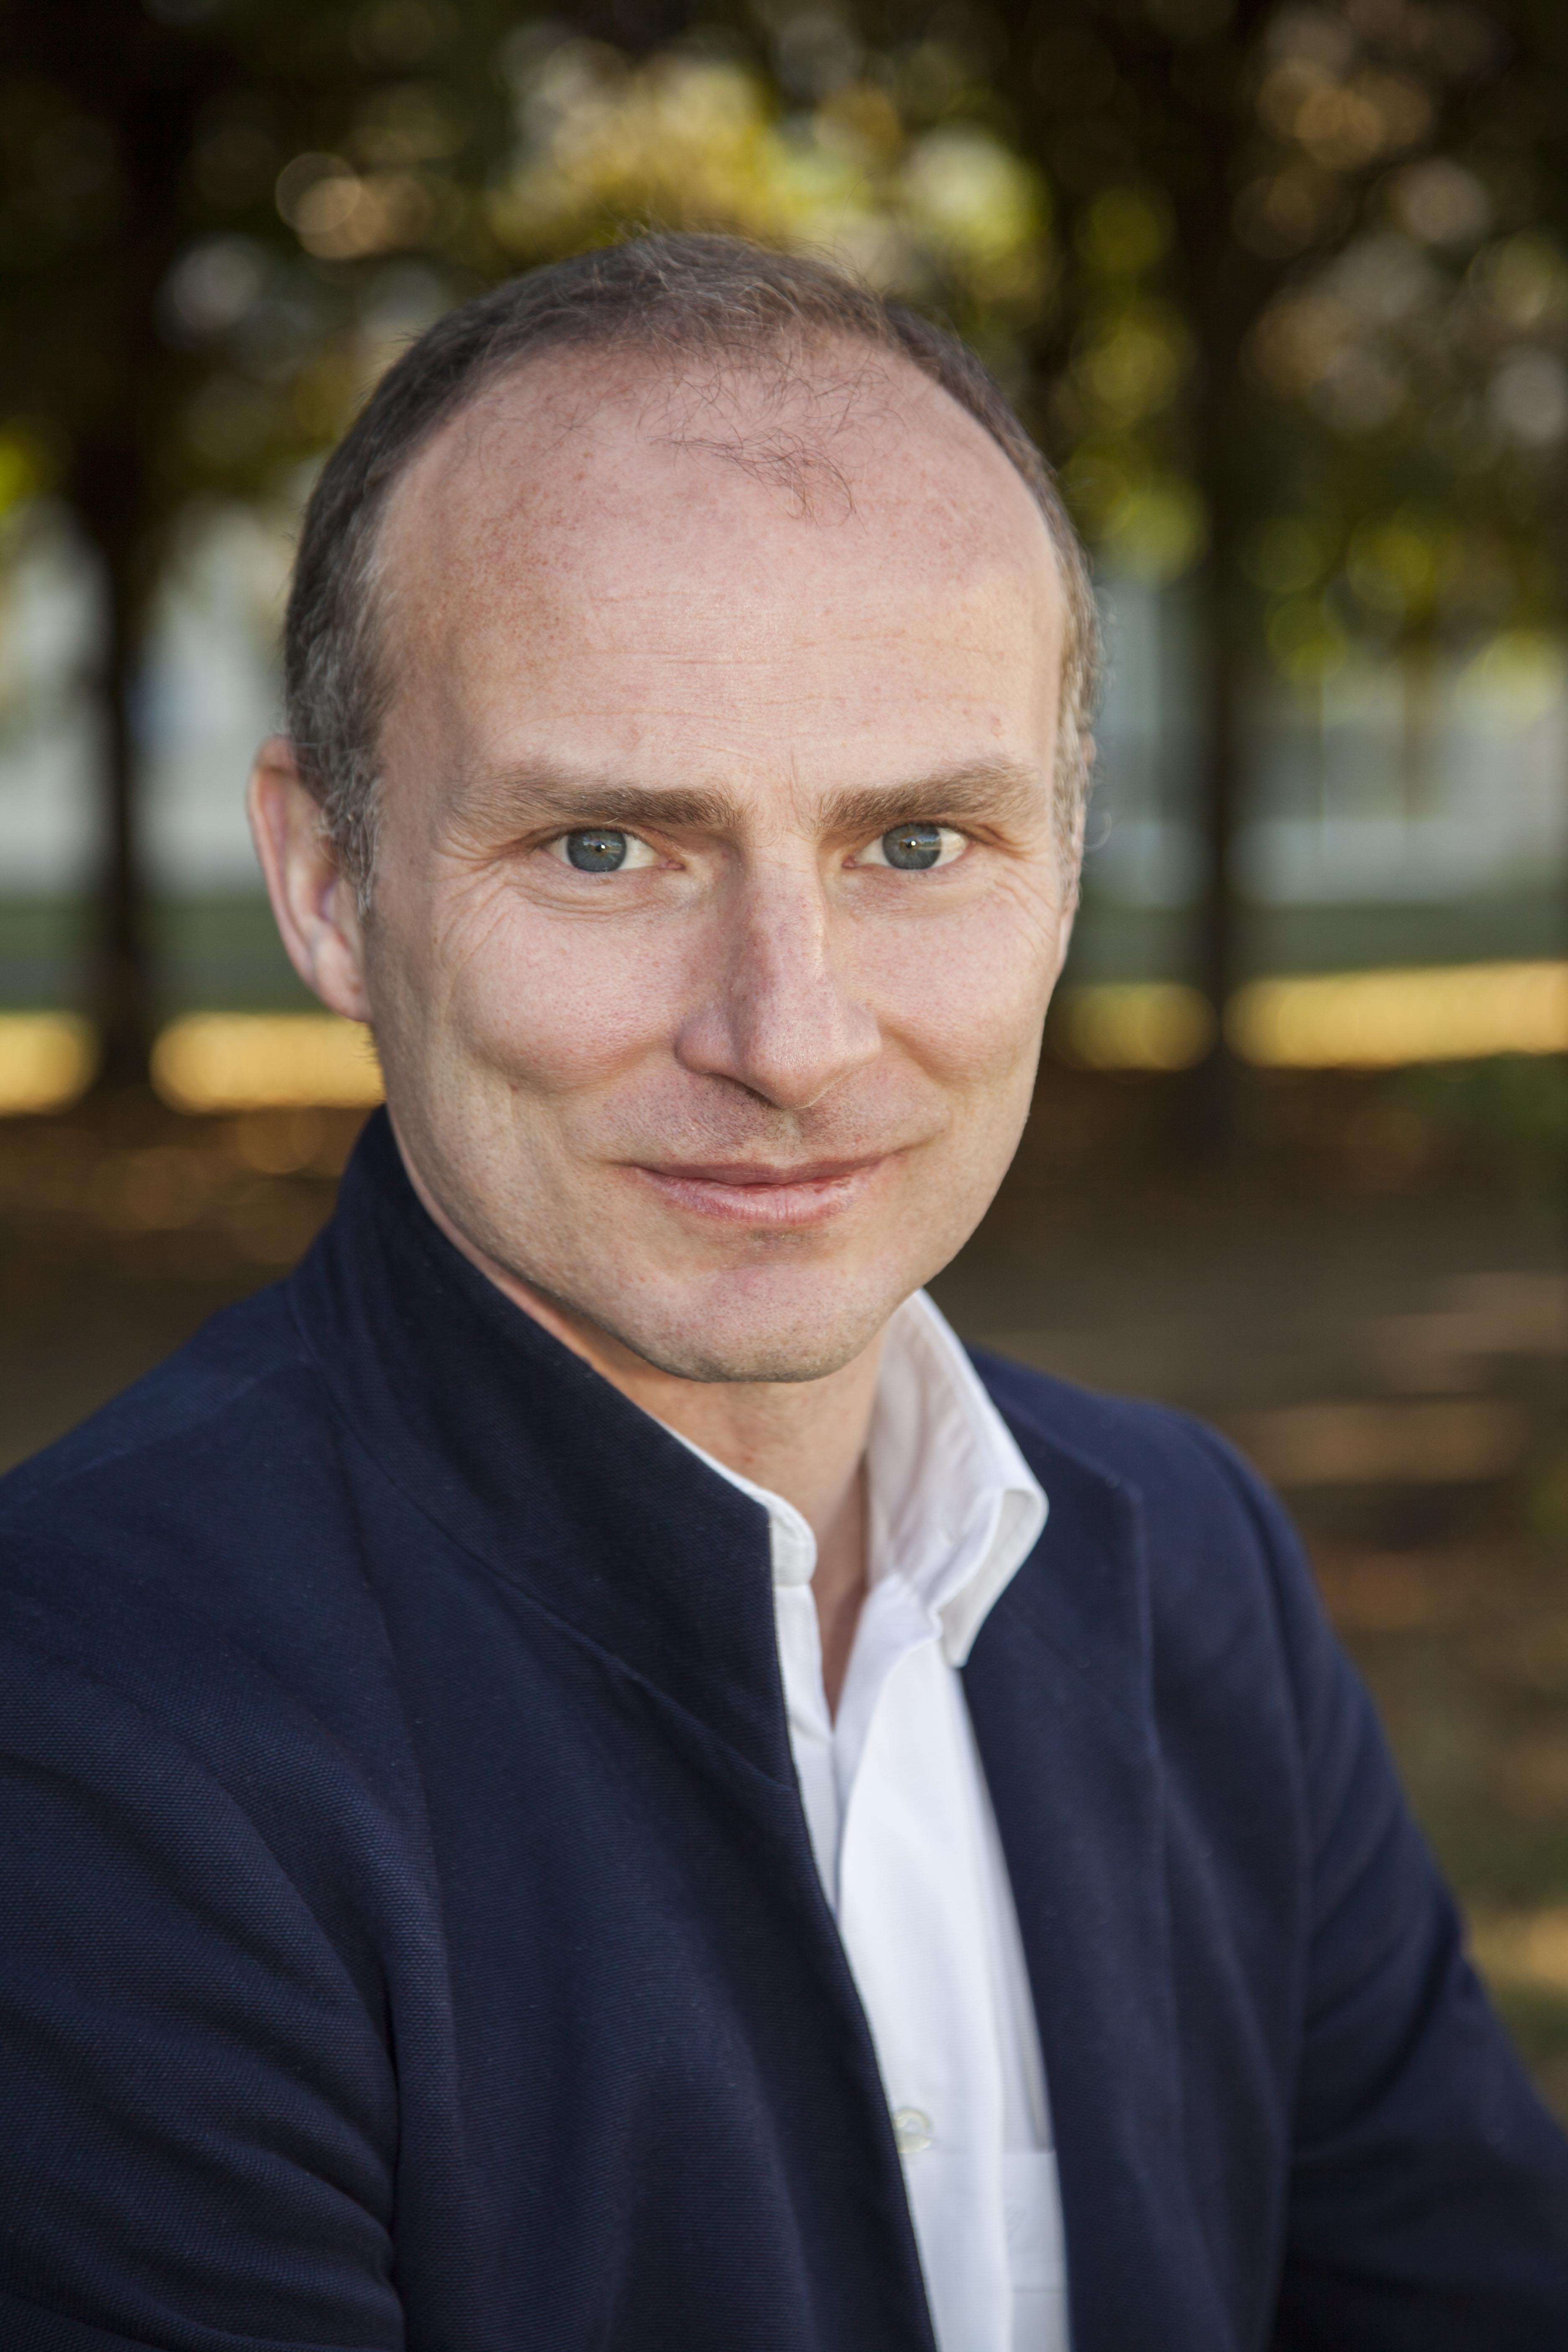
\includegraphics[height=100pt]{03PHC.jpg}
		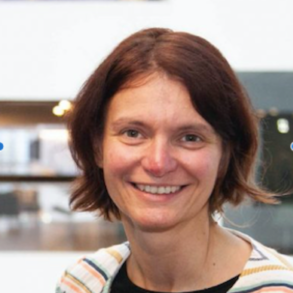
\includegraphics[height=100pt]{03CH.png}\\
		Céline and Paul-Henry
	\end{center}
	
	\textbf{How many black chocolates are behind Céline?}
	% P+C+X=50
	% 0 <= C <= 50
	% 0 <= P <= 49
	% 0 <= X <= 1
	%
	% OUT SENARIOS:
	% 1)  C=0 => X=1 ; C=50 => X=0
	% 2)  P=0 => X=1 ; P=49 => X=0
	% 3)  C=1 => X=1 ; C=49 => X=0
	% 4)  P=1 => X=1 ; P=48 => X=0
	% 5)  C=2 => X=1 ; C=48 => X=0
	% 6)  P=2 => X=1 ; P=47 => X=0
	% 7)  C=3 => X=1 ; C=47 => X=0
	% 8)  P=3 => X=1 ; P=46 => X=0
	% 9)  C=4 => X=1 ; C=46 => X=0
	% 10) P=4 => X=1 ; P=45 => X=0
	% 11) C=5 => X=1 ; C=45 => X=0
	% 12) P=5 => X=1 ; P=44 => X=0
	% 13) C=6 => X=1 ; C=44 => X=0
	% 14) P=6 => X=1 ; P=43 => X=0
	% IN SENARIO:
	% 15) C=44 => X=0
	

\end{document}